%!TEX root = project.tex

\chapter*{About this project}
\paragraph{Abstract}
A brief description of what the project is, in about two-hundred and fifty words.

\paragraph{Author}
Emmanuel Osabuehien (G00373559)

\chapter{Introduction}
\section {Meal Planning Application}

In this section, I will be giving a brief introduction into what my project is and why I have chosen to do it.\\ \\
My project is known as a Meal Planning System, this is a system that offers meals for people so they can plan and decide whats meet their dietary requirements and budget.

\begin{center}
  \begin{figure}[H]
    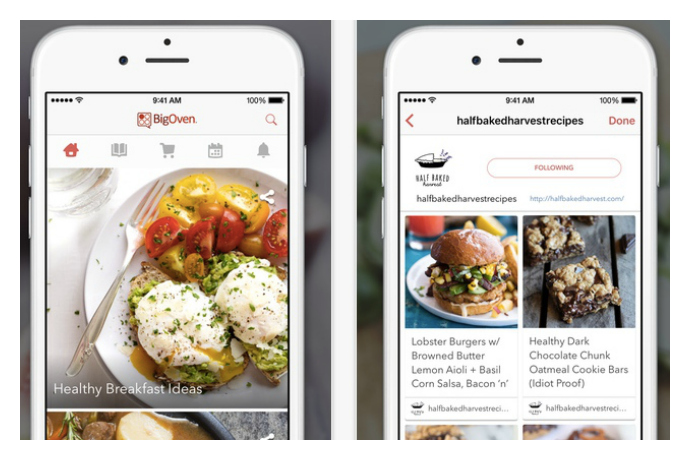
\includegraphics[width=\textwidth]{img/mealplanningpic.jpg}
    \caption{Mean Planning Example}
    \label{fig: Example of a Meal Planning System}
  \end{figure}
\end{center}

\subsection{What is a meal planning application?}

A meal planning application is an app that you plan several weeks of meal plans/grocery lists and then put those weekly meal plans into a rotation, this system is designed for users to eat healthier, giving users the decision to think about what they would like to eat and will those select items provide your body with nourishment.

\subsection{History of meal planning}

First, time devoted to cooking has decreased: in the United States, it has been reduced from 1:63 hour per day in 1965–1966 to 58 min in 2006–2007. Additionally, the source of food consumed has changed: people consume less food prepared at home, whereas foods prepared away from home represent an increasing part of the diet. \\ \\
These studies highlighted that the consumption of food prepared away from home is associated with a lower quality diet and a higher body mass index, whereas benefits have been attributed to home-prepared food. \\ \\
Previous research emphasized that individuals with lower cooking skills were more likely to consume away from home food such as ready meals or take-out meals from fast food or restaurants. \\ \\
To face time pressure, a series of qualitative studies highlighted that parents resort to food choice coping strategies, such as meal simplification, taking out, or meal planning despite their potential impact on diet quality. \\ \\
Among these strategies, time management skills and in particular meal planning, which consists in deciding ahead the foods that will be eaten in the next few days, has been previously suggested as a solution to balance competing time demands and reduce barriers to healthy dietary practices. \\ \\
Studies performed on general populations showed that meal planning was positively associated with frequencies of home food preparation and family meal, as well as the presence of fruits for dinner. \\ \\
In the present study, we hypothesize that meal planning might encourage home meal preparation, and therefore have beneficial effects on dietary quality and consequently on weight status. \\  \\
Then, we investigated the relationships between meal planning and diet quality, based on adherence to nutritional guidelines, energy, macronutrients and food group intakes, as well as food variety.

\subsection{Why am I making meal planning system?}

Q. Why have I choose an meal planning system? \\ \\
A. I believe this is completely correct in scope for my a software project as can conjure up many queries for me as a developer, examples of this may be how can I protect user information and how can I create a functional customer to supplier relationship within this software. This line of questioning is necessary as it is a much needed addition as I gain experience as a developer. I believe that this application is great as a developer as I gain a understanding from both a perspective of both a developer and user and some of the issues both can face. This application will enhance the skills all software developers should have time management, cross-platform software, database knowledge and problem solving. This type of application is needed for a variety of different users, for example myself as a student living away from home, I have now work independently and try provide for myself which is hard due to not always having to fund to go out and buy a vast amount of ingredients, this app can help from young people, people with deficiencies, people planning to lose wight, etc. with these sorts of issues.

\subsection{What are some of my issues with most meal planning systems and how do I think they can be improved?}

Many users of a typical meal planning systems depending on who you ask tend to have many problems with many modern meal planning apps, this can include apps such as 'Paprika' and 'MealBoard'. Some of the problems I will discuss below and give my take on how to combat these issues \\ \\
\textbf{Lack of Information: }Many users of meal planning apps will tell you how their is a lack of information given to a regarding nutrients the body needs.
My plan to combat this is by presenting users with a graph that shows what is the percentage of food types necessary for a person to consume in a day. \\ \\
I will also present users with recipes/meals and proper instructions into how to prepare and cook these meals instead of just giving users a list of meals they would have to research by themselves.
\\ \\
\textbf{Practicality: }I aim to provide an eye-catching user interface by using the react libraries available such as React Bootstrap, ChartJS and React Hook Form to provide users with a simple meal planning app with a navigation bar to move through different pages and providing exciting features.\\ \\
\textbf{Lack of Customization: }I aim to make this app feel personal to the user, it will involving adding graph/charts showing expenditure towards meals giving the user a very different experience than what they are used to.\\ \\
\textbf{Economic Consideration: }Most apps regarding meal planning will not take into consideration users economic struggles, which is something I believe should be always kept in mind, to combat this issue I will provide a list of meals from cheap to expensive to make so users will not be worried about their expenditure when choosing meals. 
\\ \\
\textbf{User Interface: }The user interface on most meal planning apps are not easy on the eye and quite dull. I plan to make one of more quality and vibrant to visualize for a user so they are more intrigued when they view the app. \\ \\
These apps may also be difficult to understand how to move around, I plan to make my app so it will be a quite easy to for a new user to navigate around.

\section {MERN Stack}
In this section, I will be talking about a MERN Stack, we will be going through the points of what it is, why I am using it and how is it employed.
\begin{center}
  \begin{figure}[h!]
    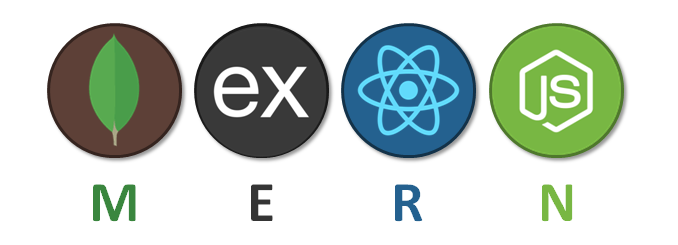
\includegraphics[width=\textwidth]{img/mern-stack.png}
    \caption{MERN Stack Logo}
    \label{fig: MERN Stack Image}
  \end{figure}
\end{center}
Now to put everything into context MERN is an acronym made up of the key technologies that make up the stack itself.
\begin{itemize}
\item M = MongoDB
\item E = ExpressJS
\item R = ReactJS
\item N = NodeJS
\end{itemize}
This is a big reason why I chose to use a MERN Stack for my project as this technology provides a smooth, simple way to make a full-stack web application that can be explained as follows. \\ \\
\textbf{MongoDB} is a open source, cross platform, NoSQL document-oriented database which is used to store a large amount of data in documents and collections. \\ \\
\textbf{ExpressJS} is server-side, back end web application framework that is used for NodeJS needed to write simple and secure applications. \\ \\
\textbf{ReactJS} is a open source, front end JavaScript Library used to create graphical user interfaces of web applications. \\ \\
\textbf{NodeJS} is a open source, cross platform back end JavaScript run time environment, running the JavaScript code outward of the browser. \\ \\

\subsection{MongoDB}

\begin{figure}[H]
  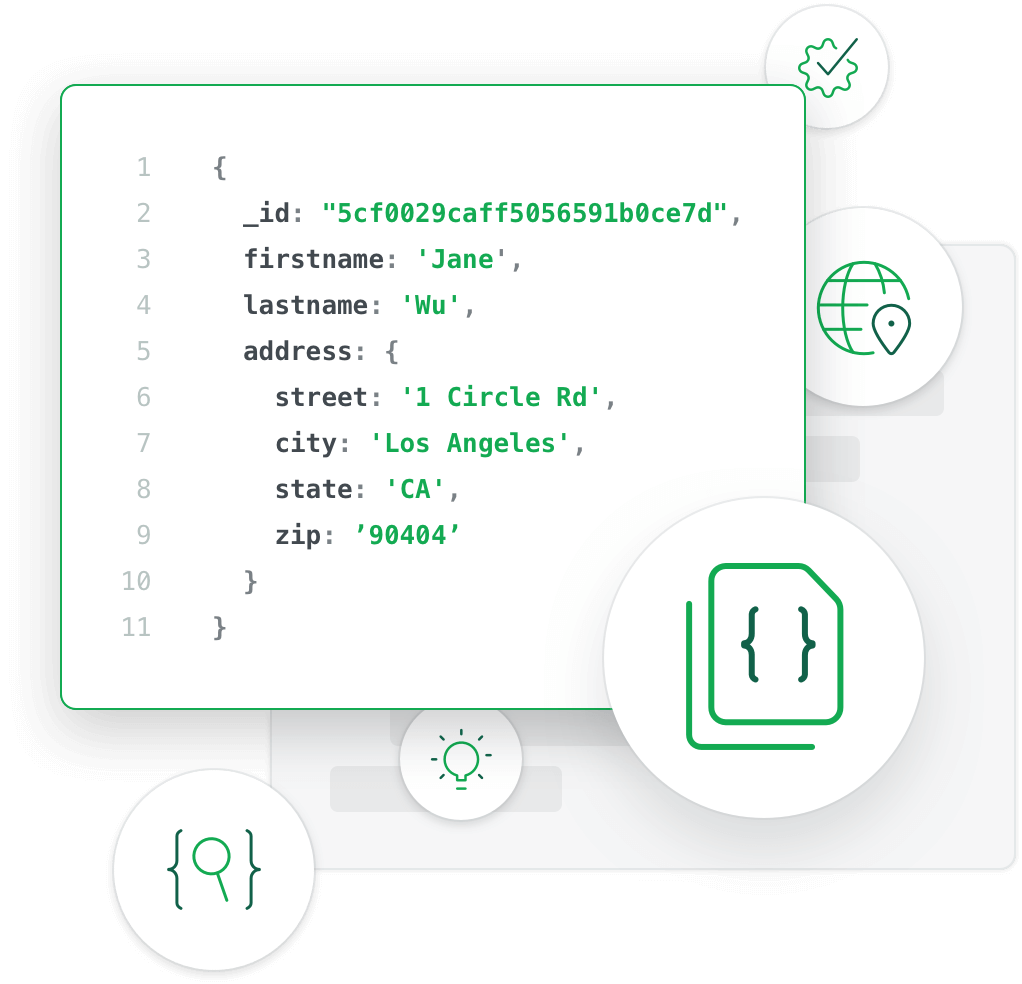
\includegraphics[scale=0.35]{img/mongodbeg.png}
  \centering
  \caption{Example of Mongo Database}
  \label{fig: Mongo Database}
\end{figure}

The reason I decided to use MongoDB as opposed to MySQL or other services available for my database management can be broken down into a couple of reasons, one of the big reasons is it's growth in popularity but removing that key factor MongoDB has many advantages over most services in this area including:

\begin{itemize}
\item\textbf{MongoDB} can handle large volumes of unstructured data
\item\textbf{MongoDB} has the ability to scale up quickly
\item\textbf{MongoDB} allows schemas to be flexibile due to it's data models
\item\textbf{MongoDB} is constantly evolving
\end{itemize}

\subsection{ExpressJS}

\begin{figure}[H]
  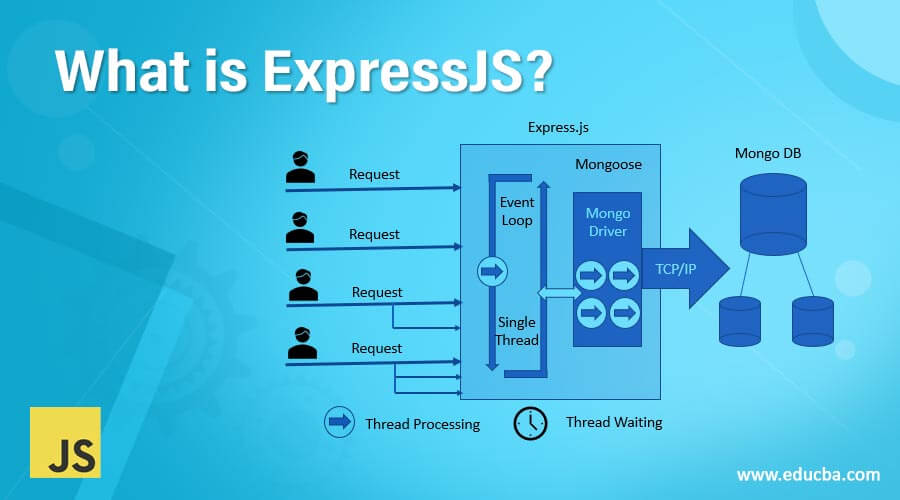
\includegraphics[scale=0.4]{img/whatisexpressjs.jpg}
  \centering
  \caption{Example of an ExpressJS process}
  \label{fig: What is ExpressJS?}
\end{figure}

The reason I chose ExpressJS as opposed to other frameworks for my back end development is due to it's high quality status of performing a server-side connection and it's ability for unfamiliar users to easily use, learn and understand, other positives include:

\begin{itemize}
\item\textbf{ExpressJS} allows users to use the same programming language as the front end
\item\textbf{ExpressJS} has the ability to scale your application quickly
\item\textbf{ExpressJS} can easily connect to databases such as MongoDB or MySQL
\item\textbf{ExpressJS} works well with NodeJS
\end{itemize}

\subsection{ReactJS}

\begin{figure}[H]
  
\includegraphics[scale=1.0]{img/reatcjspic.png}
  \centering
  \caption{Example of React App Symbol}
  \label{fig: React App Symbol}
\end{figure}

The reason I chose ReactJS as it is a JavaScript library that is great for building user interfaces and framework that has been on the rise since it's conception in 2013, ReactJS offers many services and features when creating an easy to navigate user interface, other advantages include:

\begin{itemize}
\item\textbf{ReactJS} is easy to use and understand
\item\textbf{ReactJS} provides reusable components of HTML code
\item\textbf{ReactJS} offers a scope where developer can test and debug code
\end{itemize}

\subsection{NodeJS}

\begin{figure}[H]
  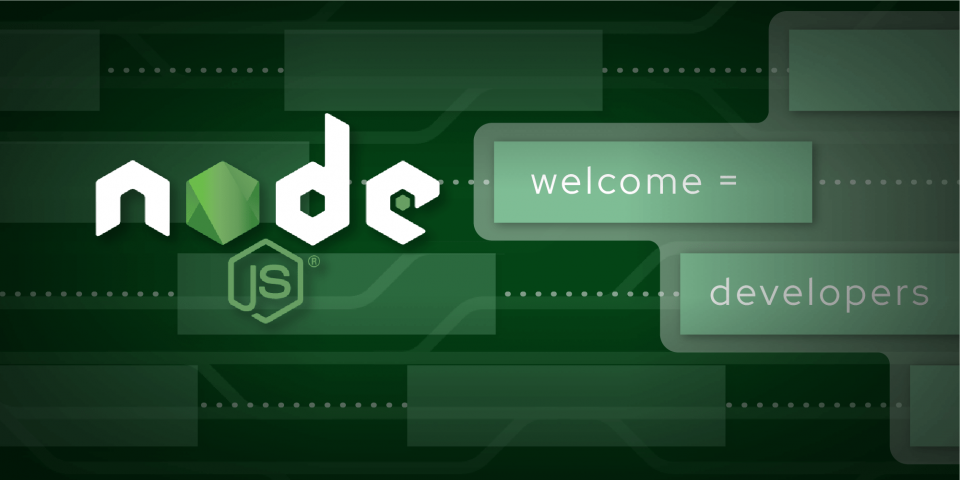
\includegraphics[scale=0.5]{img/nodejspic.png}
  \centering
  \caption{Image of NodeJS Background}
  \label{fig: NodeJS Background}
\end{figure}

The reason I chose NodeJS because it because of server-side security, what it also offers, which includes various tools and libraries useful in web applications and it's ability to easy handle server-side requests, other advantages include:

\begin{itemize}
\item\textbf{NodeJS} has the ability to scale up quickly
\item\textbf{NodeJS} is a very flexible run time environment
\item\textbf{NodeJS} is easy to use, learn and understand
\item\textbf{NodeJS} offers cross-platform development, for example you can connect a mobile app link to a desktop app
\end{itemize}

\section{Positives and Negatives of Meal Planning Systems}

In this section, I will discuss both the positives and negatives of meal planning applications

\subsection{Positives}

\begin{itemize}
\item Aiming for weight loss goals
\item Easy to prepare for shopping
\item Allows for better money management
\item Saves users time and energy
\item System offers users a wide variety of ideas to use
\item It might be able to offer some nutritional knowledge
\end{itemize}

\subsection{Negatives}

\begin{itemize}
\item Recipes may not be up to user satisfaction
\item It means setting a schedule and plan and sticking as close to it as possible
\item It takes planning and discipline to meal plan, that you might not have
\item Inflexible and don’t account for varying needs of the body
\end{itemize}

\section{The Benefits of Meal Planning Systems}

In this section, I will discuss the benefits of a meal planning application

\subsection{Health Goals}

 Cooking meals at home increases your chance of reaching health goals, whether or not they are planned to lose weight, improve heart health or keep blood sugar steady, meal planning is what gives you ingredients and resources to actually make this happen on a daily basis.

\subsection{Budgeting}

Meal planning makes it easier to cook more at home, and shoppers can save even more by weekly sales into planning. So the next time you're budgeting for an expense, consider meal planning to help save you money on a set basis.

\subsection{Enables Variety and Gives Control}

Meal planning is often associated with increased food variety, which is key to  a healthy diet that increases your goal of meeting nutritional needs.

Meal Planning also gives you control and choice over ingredients as it is easier to avoid food allergens and to incorporate ingredients that support diets for specific health problems

\subsection{Streamlines Shopping and Decreases Food Waste}

Meal planning allows users to set out their list of ingredients to obtain based around their meal plan, reducing the time and money spent to constant shopping trips.

You are also most likely to make use of forgotten food items that are just stored away, reducing the amount of food waste and unneeded shopping trips by utilizing what you already have on hand.

\subsection{Decision Fatigue}

Meal Planning helps to alleviate the stress and fatigue when deciding what to meals you need to make throughout the day as users can stock up ingredients and have multiple planned meals where they have a wide variety of options to choose from.

\section{Software Requirements}

In this section, I will give a list of the software requirements I intend my project to achieve

\begin{itemize}
\item\textbf{Login: }If user has an account, they are required to login to use application
\item\textbf{Register: }If users don't have an account, they are required to register an account and login to use application
\item\textbf{Logout: }Users can logout if application is not in use
\item\textbf{Forget Password: }If users can't access account/forgot their password, they can retrieve their account by following process provided
\item\textbf{Add Meal: }Uses can add meal into the listing page
\item\textbf{List All Meals: }Users can access listing page where they can view all meals that have been added
\item\textbf{Fetch Meal: }Users can retrieve the meal that they have added to the listing page
\item\textbf{Delete Meal: }Users can delete the meal that they have added to the listing page
\item\textbf{Edit Meal: }Users can update the meal that they have added to the listing page
\item\textbf{Cookies: }The application must use cookies to memorize information during visits and maintain sessions.
time-frame max of a day.
\item\textbf{Security: }Users login details must be encrypted and secure so they cannot be accessed by another user
\end{itemize}

\chapter{Context}

\section {Objectives}

In this section, I will discuss the key objectives that I intend to carry out for this web application. \\ \\
The objectives include:

\begin{itemize}
\item To create a multi-user, functioning web application that can be accessed
\item To an attractive, simple and easy to understand graphical user interface that users can operate without difficulty
\item To provide a system where users can plan out their meals
\item To provide users a system keep track of dietary goals
\item To provide users with nutritional education
\item To provide a multi-user app with a secure database of users where login details are encrypted
\item To provide a REST API to my service to allow users to perform requests
\end{itemize}

\section {Overview of Chapters}

In this section, I will give a brief overview of what each chapter in my dissertation contains.

\subsection{Introduction}

In this chapter, this is just an introduction of the project, where we what is the project, why I choose to make this project and use the technology I utilized, provides what are the key objectives of this project and give the viewer an idea on what this dissertation contains.

\subsection{Context}

As is evident by the title of this chapter, in this chapter I will discuss the context of my project, the importance and rise of web-based issue ticketing systems, the benefits and drawbacks of meal planning apps and how convenient they came to be in modern computer science especially in a software project collaborative setting.

\subsection{Methodology}

In this chapter, I will discuss my approach to this project, the methodology and testing I used for this project and why I chose a certain type of methodology and testing, how this had an effect on my project and go into more detail on how the developmental process of my project

\subsection{Technology Review}

In this chapter, I will discuss more about the technical features of the project, all the technologies used in my project at a more conceptual level, how did they affect the developmental process, why did I choose this technology to implement and should a good indication of the research that was undertaken during the creation of the project.

\subsection{System Design}

In this chapter, I will give a detailed explanation of the system architecture i.e., Front End, Back End, Database. There will be an overview of the different components of the system and how they function together when deployed and diagrams to explain and visualize the design of the system.

\subsection{System Evaluation}

In this chapter, I will give an evaluation of my project against the objectives I set out for myself and I will test whether the project meets the user requirements and quality standard. This chapter will include testing of the stability and behaviour of the software and provide graphs/table of the results.

\subsection{Conclusion}

In this chapter, I will summarise various points of the project, I will outline the context, the set objectives and if this was satisfactory to the goals i set for myself. I will discuss the research conducted and highlight the findings I discovered through that process. I will also finally give a list of outcome of the project.

\section {Project Structure}

In this section, I will give a brief overview of the structure of my GitHub repository for viewers.
\begin{figure}[H]
  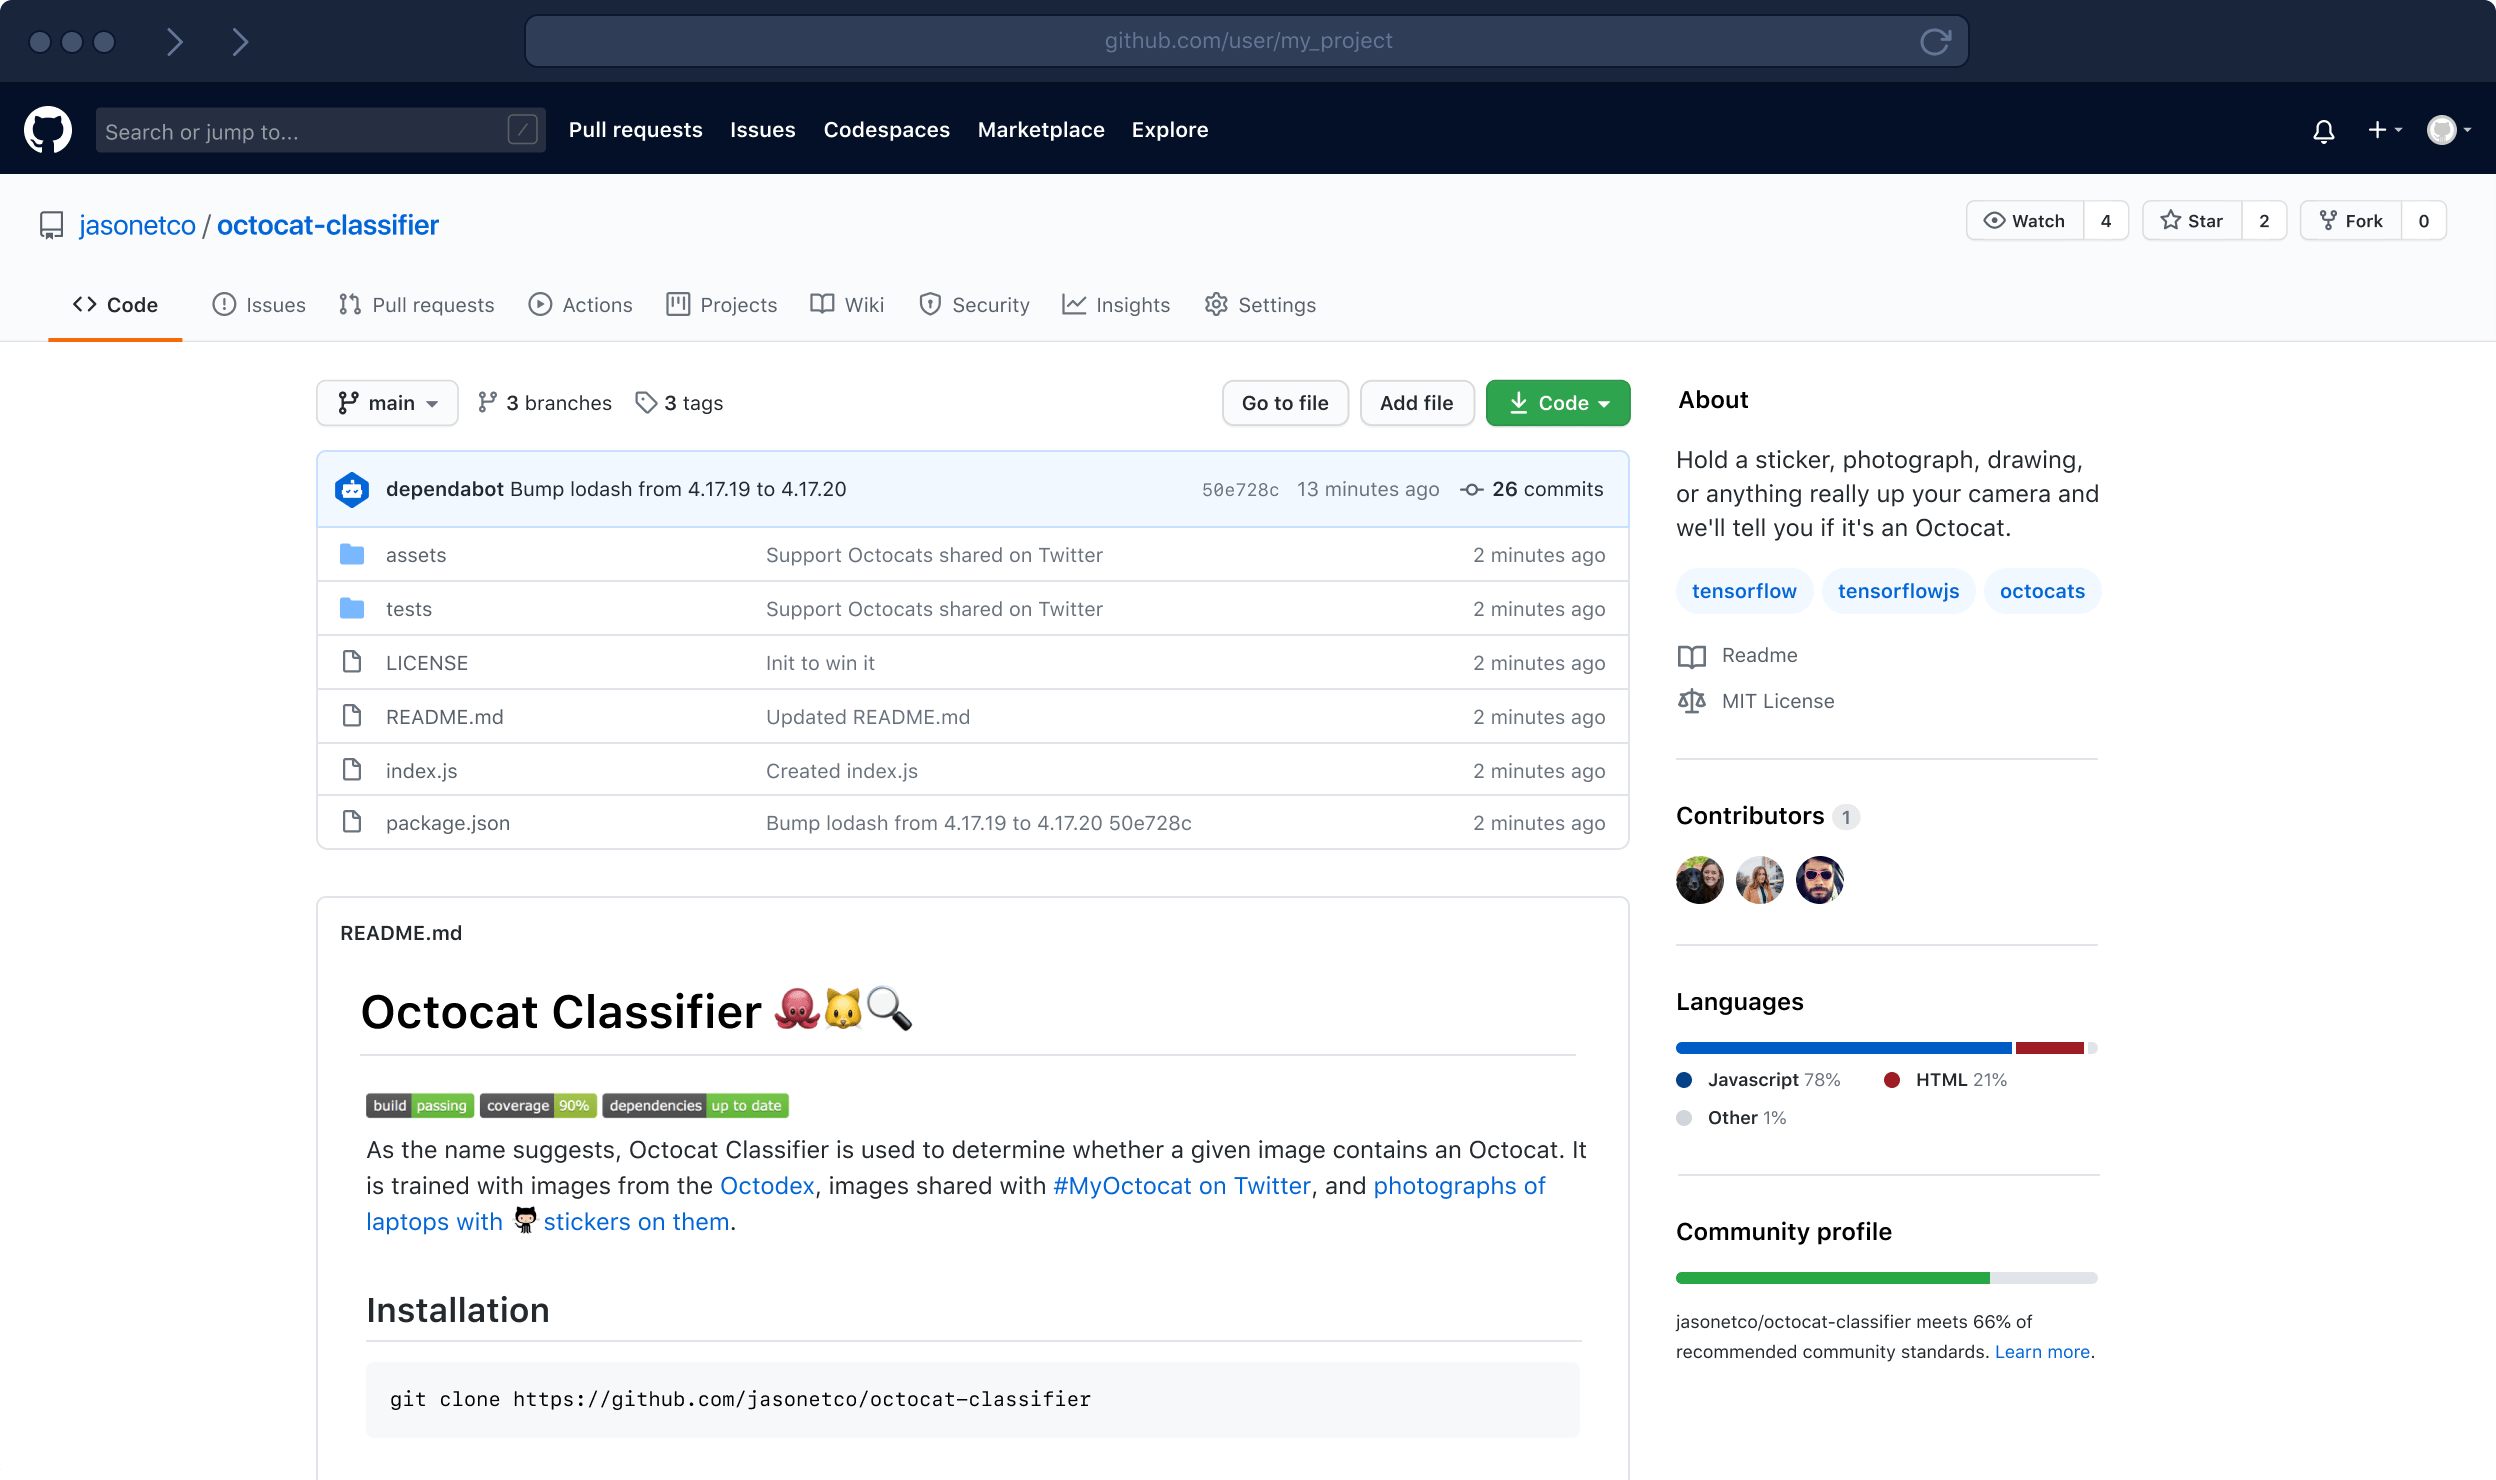
\includegraphics[scale=0.15]{img/githubpic.png}
  \centering
  \caption{Example of GitHub Repository}
  \label{fig: GitHub Repo Example}
\end{figure}
The GitHub repository where this project is located in contains two specific folder, my 'meal-planning' folder which contains the main application of the project (including the front end and back end of my application) and the 'img' folder which contains images used in my application. \\ \\
Apart from this folder my project also contains the files for the dissertation including the 'content.tex', 'project.tex', 'bibliography.bib', the project.tex which contains the cover sheet of the dissertation, content.tex which contains the chapters and sections written and the bibliography.bib which contains the primary, secondary and tertiary resources that are cited in the dissertation. \\ \\ 
There is a README.md file which contains information on why this repository exists, what is in it and how to run the project.  \\  \\
There is also a LICENSE.txt file which is used as a software license agreement. \\ \\
You can view the github by clicking the link as follows: \\  \\ \url{https://github.com/Emmanuel-Osabuehien/AppliedProjectMinorDissertation}

\chapter{Methodology}

\section{Overview}

In this section, I will give a quick overview on what is Methodology.\\ \\
During the process of creation my application, I research different approaches, testing and validation to keep my project organized. I adopted the Agile (incremental and iterative) approach for my project, I set up sprints where I set up tasks needed to be completed in a two week period. I also used Test Driven Development (Selenium and JUnit) where I wrote tests with enough code to allow it to pass without bugs, error and fault which I will later on edit this very same code.

\section{Agile Methodology}

In this section, I will discuss what is methodology, different types of methodology and how I implemented methodology in my project.

\subsection{What is Agile Methodology}

Agile is both an incremental and iterative approach to project management and software development that helps teams deliver value to their customers faster according to 'Atlassin', one of the leading examples of Agile framework. Scrum, DevOps, Trello and Jira are only a few examples. The Agile Manifesto outlines the principles that all Agile techniques follow. I'll be utilizing Trello for the duration of this project. Continuous improvement and incremental delivery are key to all Agile approaches.

\begin{figure}[H]
  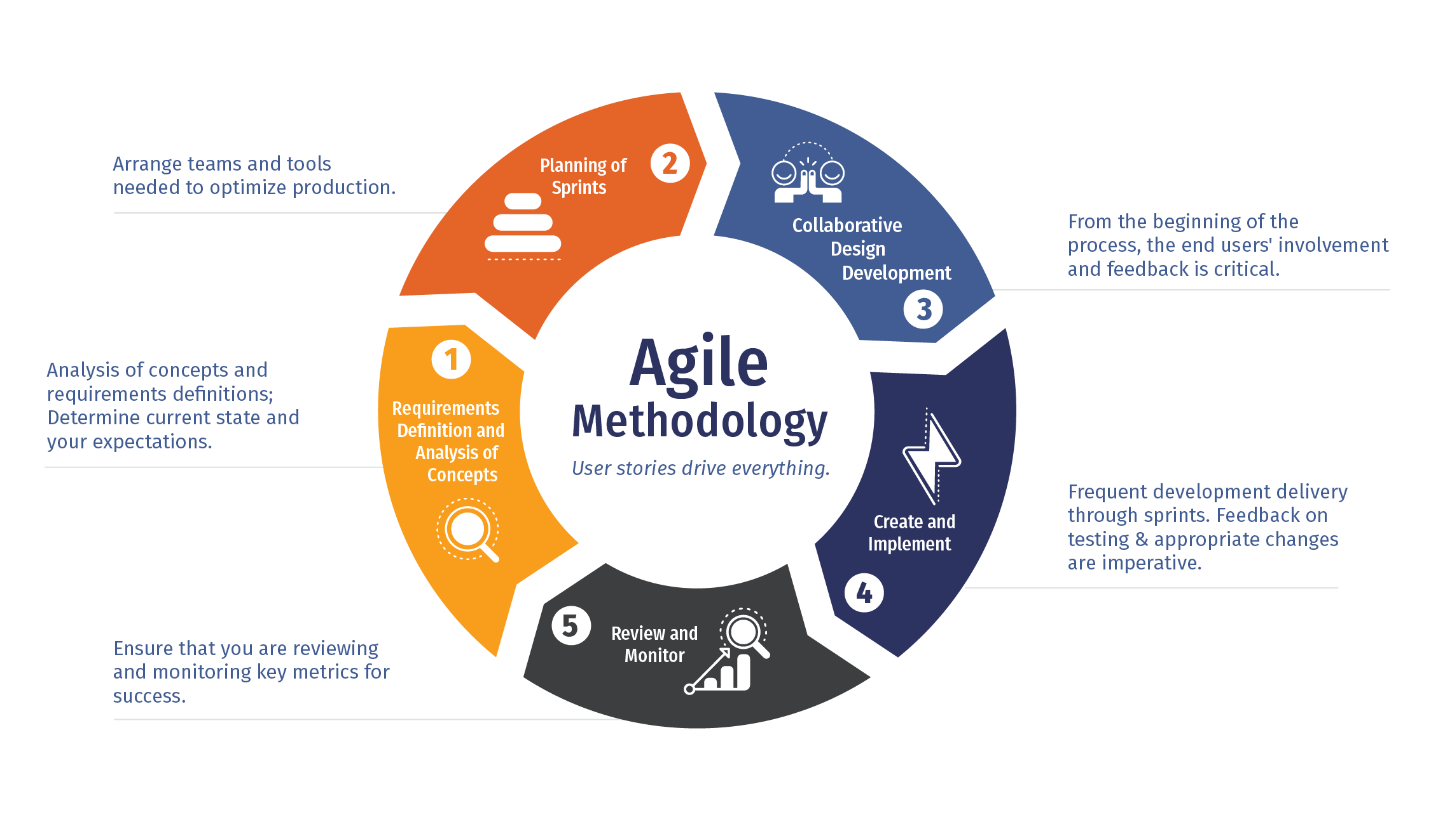
\includegraphics[width=\textwidth]{img/agilemeth.png}
  \caption{Agile Methodology}
  \label{fig: Agile Lifecycle}
\end{figure}

\subsection{Atlassian}

Q. Why did I choose Atlassian as my Agile framework?\\ \\
\begin{wrapfigure}{r}{0.5\textwidth}
  \begin{center}
    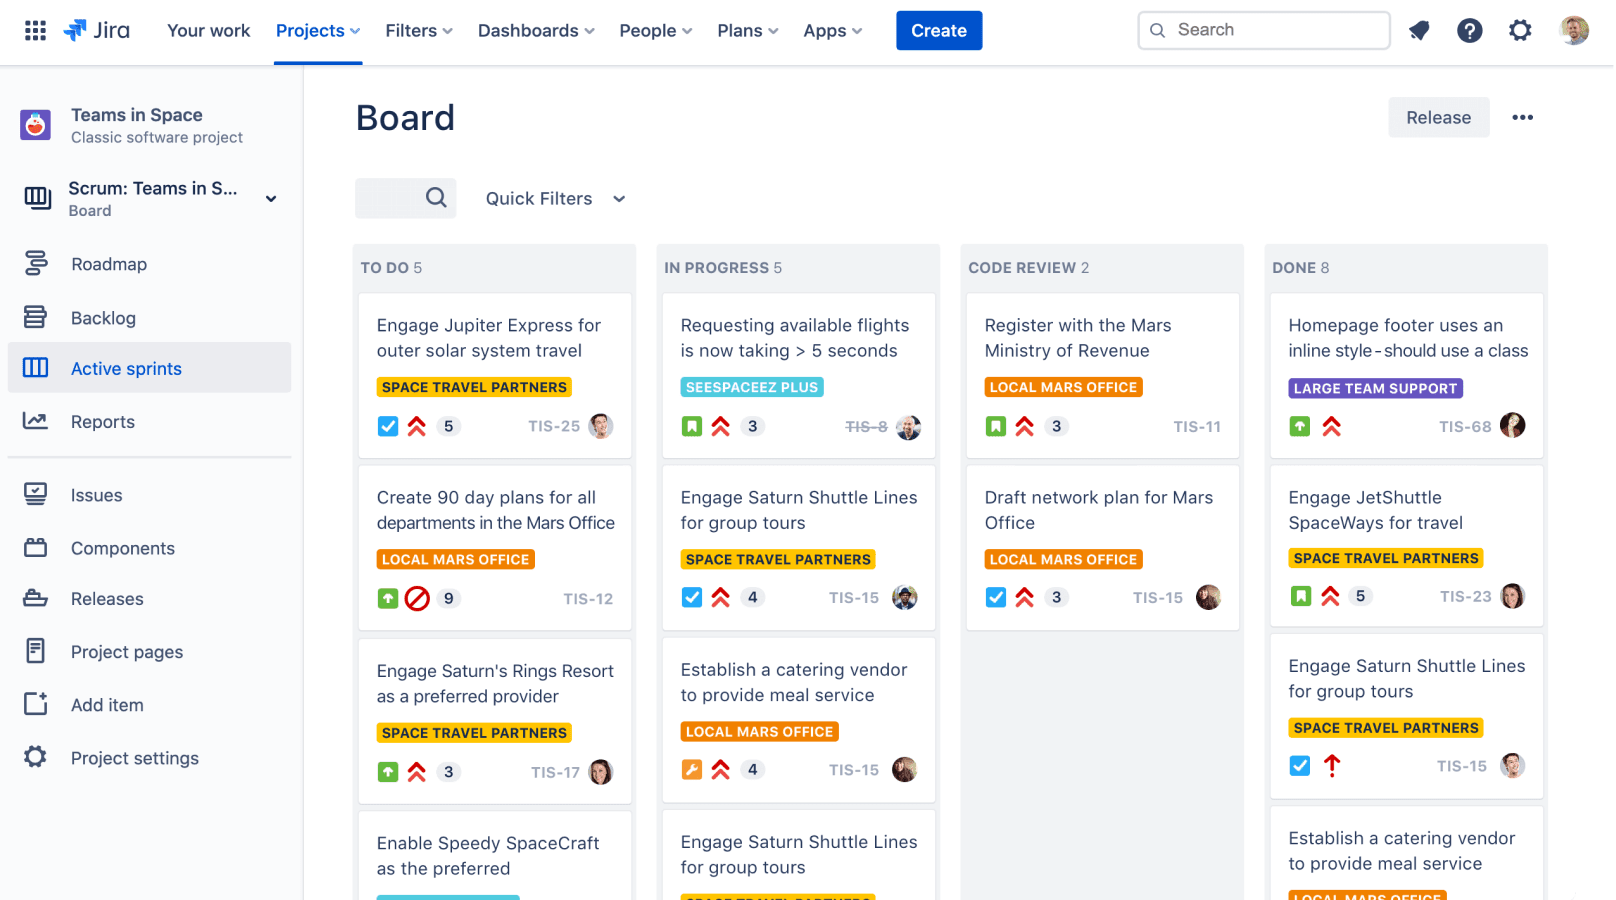
\includegraphics[width=0.75\textwidth]{img/atlasboard.png}
  \end{center}
  \caption{Atlassian Board}
  \label{fig:Example of Atlassian board}
\end{wrapfigure}
A. Atlassian gives the user (or a team) a clear view into the status, progress, and success of projects.  Also, they issue Power Ups to help you work across boards, with an visually appealing user interface.\\ \\
Atlassian also offers features such as:

\begin{itemize}
\item Following production workflow
\item Organizing future projects
\item Keeping track of project developmental process
\item Managing development schedule
\end{itemize}

\subsection{Implementation}

I implemented Trello with my project by connecting my GitHub repository to my project and I set up my sprints in my backlog and added tasks that were to be completed to my working board. I created 3 sections to my board for my working project known as "To Do", "Doing" and "Done", 'To Do' contained issues that were just added, 'Doing' contained issues that are in progress of being completed and 'Done' contained issues that were completed. This helps with the output, outcome and productivity of my project as I can visualize what I need to do and work on in a set schedule. I also have 2 other sections "Backlog" and "Issues", "Backlog" contains all functionality desired in the product and "Issues" contains any bugs, errors or fault in code that needs to be checked.

\section{Validation and Testing}

In this section, I will discuss validation and testing, what they are in terms of software development, different types of software that supply validation and testing and how I implemented testing in my project.

\subsection{Test Driven Development}

Test Driven Development (TDD) is software development approach in which test cases for each functionality are created and tested first and if the test fails then the new code is written in order to pass the test and making code simple and bug-free.

\subsection{Implementation}

I designed and wrote test cases whenever I developed a code to perform a specific functions for my application such as a 'Add a meal to your list' or 'Delete a meal that you have added to the list', after this test was performed I wrote a significant amount of code so the test should not fail and pass and continued to edit the code.

\subsection{Regression Testing}

Regression Testing is a type of software testing to confirm that a recent program or code change has not had a detrimental affect to the existing features of an application.\\ \\
Regression Testing is a selection of already executed test cases which are re-executed to ensure existing features and functionalities of the running application works as intended to and that their are no bugs, errors or faults.\\ \\
This testing is applied to make sure that new code changes do not cause any bugs, errors or faults to the existing features and functionalities. Ensuring the old code still functions as normal in the wake of the new code changes.

\subsection{JUnit}

JUnit is just one of the testing frameworks I used to perform automated tests. JUnit is a open-source framework, it is used to write and run repeatable automated tests. JUnit is used to perform Java tests and is one of the leading examples of regression testing. This allowed me test the database functions to make sure when the code is run it works smoothly and also make sure certain outputs were correct such as 'Tallying the shopping list cost'.

\begin{figure}[H]
  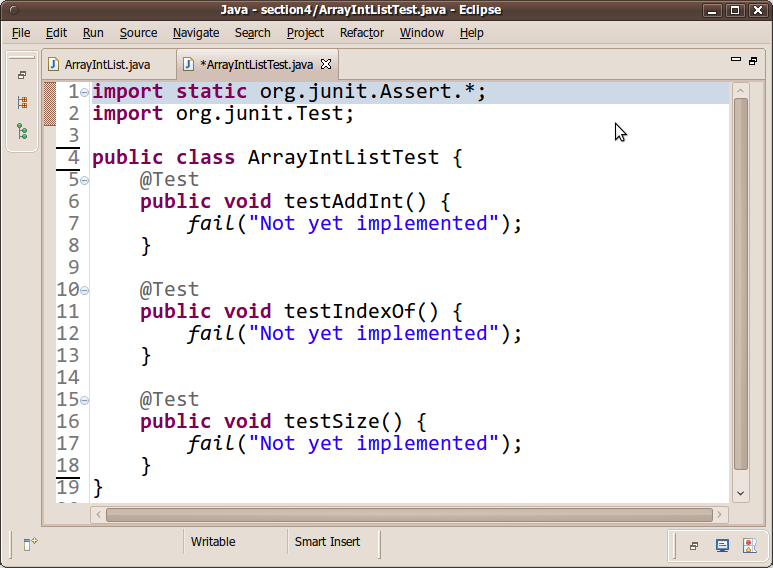
\includegraphics[width=\textwidth]{img/junitcase.png}
  \caption{Example of JUnit 5 Test Case}
  \label{fig: JUnit Test Case}
\end{figure}

\subsection{Selenium}

I also used Selenium to perform automated tests for my application. 
Selenium is a open-source automated testing framework used to validate web applications across different browsers and platforms that can be used for multiple programming languages such as Java, JavaScript, Python, etc. 
Selenium is used to perform automation testing on such user interfaces and web pages, I implemented Selenium in my React application using Node and this allowed to test the database functions to make sure when the code is run it works smoothly.

\begin{figure}[H]
 \begin{center}
  
\includegraphics[scale=0.25]{img/seleniumlogo.png}
  \end{center}
  \caption{Selenium Logo}
  \label{fig: Image of Selenium Logo}
\end{figure}

\section{GitHub}

In this section, I will discuss the importance of GitHub during the development of my project. \\ \\
GitHub and Git were both very important in the development of my project. I used GitHub to manage all my files and folders regarding my project, repeatedly pushing these files/folders to GitHub whenever progress was made. I used GitHub with my Trello Boards where I would manage issues that arose during the development stages.\\ \\
\begin{wrapfigure}{r}{0.5\textwidth}
  \begin{center}
    
\includegraphics[width=0.35\textwidth]{img/githublogo.png}
  \end{center}
  \caption{GitHub Logo}
  \label{fig:Image of GitHub Logo}
\end{wrapfigure}
GitHub also allowed to me to use multiple branches where I created separate branches 'Main' and 'Master' where I would use Main for my finished code that had been tested and 'Master' for tested certain features which allowed me freedom to perform automated tests for debugging my application. \\ \\
GitHub also provides me with the option of return to previous iterations of my project, so in the case of an errors in the system I can just start again from a previous working and tested version as well as a page dedicated to issues where I can post issues that would then be divided into 2 week sprints.

\section{Issues Faced}

In this section, I will discuss the issues that I faced during the development of my project.

\subsection{Project Timeline}

The project timeline (or organization) was one of the issues I faced during the development of my project as dealing with a variety of different projects and trying to balance them all together was a difficult task that I had to solve. I solved this issue by creating a weekly schedule where I would allocate a select amount of time for different modules and project that I was working on so I didn't focus and stress about one project more than another.

\subsection{Underestimating The Scope}

The project scope was another issue I faced as I went through several ideas for my project and struggled with identifying if any of those ideas was the correct scope for my project. I overcame this obstacle by having weekly meetings with my supervisor where we would discuss on if the scope of my idea was right until coming to a conclusion.

\subsection{Feature Overload}

Feature overload was another issue that was faced during the development of my project as trying to select the right software/technology was difficult as I stressed how multiple types of software would gel together until I decided to use a MERN Stack that all flowed together smoothly and worked well together.

\chapter{Technology Review}
About seven to ten pages.
\begin{itemize}
\item Describe each of the technologies you used at a conceptual level. Standards, Database Model (e.g. MongoDB, CouchDB), XMl, WSDL, JSON, JAXP.
\item Use references (IEEE format, e.g. [1]), Books, Papers, URLs (timestamp) – sources should be authoritative. 
\end{itemize}

\section{XML}
Here's some nicely formatted XML:
\begin{minted}{xml}
<this>
  <looks lookswhat="good">
    Good
  </looks>
</this>
\end{minted}

\chapter{System Design}
As many pages as needed.
\begin{itemize}
\item Architecture, UML etc. An overview of the different components of the system. Diagrams etc… Screen shots etc.
\end{itemize}
\begin{table}[h]
  \centering
  \begin{tabular}{x{2cm}p{3cm}}
    \toprule \\
    Column 1 & Column 2 \\
    \midrule \\
    Rows 2.1 & Row 2.2 \\
    \bottomrule
  \end{tabular}
  \caption{A table.}
  \label{table:mytable}
\end{table}

\chapter{System Evaluation}
As many pages as needed.
\begin{itemize}
\item Prove that your software is robust. How? Testing etc. 
\item Use performance benchmarks (space and time) if algorithmic.
\item Measure the outcomes / outputs of your system / software against the objectives from the Introduction.
\item Highlight any limitations or opportuni-ties in your approach or technologies used.
\end{itemize}

\chapter{Conclusion}
About three pages.
\begin{itemize}
\item Briefly summarise your context and ob-jectives (a few lines).
\item Highlight your findings from the evalua-tion section / chapter and any opportuni-ties identified.
\end{itemize}